% !TeX spellcheck = cs_CZ
%---------------------------------------------------------------------------------------------------
% file filter.tex
%---------------------------------------------------------------------------------------------------
%==================Kapitola: Kmitočtové filtry======================================================
\setchaptertoc
\chapter{Kmitočtové filtry}

  \section{Kmitočtové filtry a jejich použití}
    Kmitočtové filtry jsou lineární elektrické obvody, používané v mnoha oblastech elektrotechniky a
    elektroniky. Jejich hlavním úkolem je \emph{výběr} (selekce) \emph{kmitočtových složek}
    procházejícího signálu podle jejich kmitočtů. Filtry obvykle některé kmitočtové složky signálů
    \emph{propouštějí} bez útlumu (oblast se nazývá propustným pásmem), jiné kmitočtové složky
    \emph{potlačují} (pásmo potlačení, útlumu, nebo nepropustné pásmo). Tyto vlastnosti obvykle
    vyjadřujeme \emph{modulovou (amplitudovou) kmitočtovou charakteristikou} (závislost modulu
    napěťového přenosu na kmitočtu).

    Příklad použití kmitočtového filtru ukazuje názorně obr. \ref{aes:fig007}. Užitečný obdélníkový
    signál byl znehodnocen nízkofrekvenční rušivou harmonickou složkou (pronikající např. z
    napájecí střídavé sítě - kmitočet sítě je nižší, než kmitočty užitečných složek), signál je
    označen v grafu jako \(u_1(t)\). Jak je z obrázku vidět, filtr typu horní propust propustil
    všechny kmitočtové složky s mezním kmitočtem vyšším než \(f_M\) (složky obdélníkového signálu) a
    potlačil tak nízkofrekvenční rušivou harmonickou složku, výsledný signál je v grafu označen jako
    \(u_2(t)\). Z obr \ref{aes:fig007} je zřejmé, že vliv kmitočtových filtrů na signál je dobře
    patrný zvláště při znázornění procesu filtrace v kmitočtové oblasti pomoci kmitočtového spektra
    - tedy pomoci rozkladu signálu na jeho jednotlivé harmonické složky.

    Průchod signálu filtrem vede též obvykle k \emph{časovému zpoždění signálu}, což je důsledkem
    fázových posuvů (zpoždění) procházejících harmonických kmitočtových složek signálu. Tyto vlivy
    obvykle vyjadřujeme \emph{fázovou kmitočtovou charakteristikou}. Jejich vliv na výstupní signál
    je též zřejmý při znázornění signálu a vlastností filtru v \emph{časové oblasti} (např. odezva
    na jednotkový skok). Fázové vlivy filtru na signál v propustném kmitočtovém pásmu se v časové
    oblasti projevují např. jako nežádoucí překmity či zvlnění průběhu signálu. V příkladu z obr.
    \ref{aes:fig007} (filtr typu horní propust) způsobil tento efekt zešikmení horních a spodních
    hran obdélníkového signálu. Uvedené vlivy je možné vhodnou volbou filtru minimalizovat. Na druhé
    straně ale existují případy, kdy těchto vlastností filtrů záměrné využíváme, např. ve fázovacích
    a zpožďovacích obvodech.

    \begin{figure*}[ht!]
      \centering
      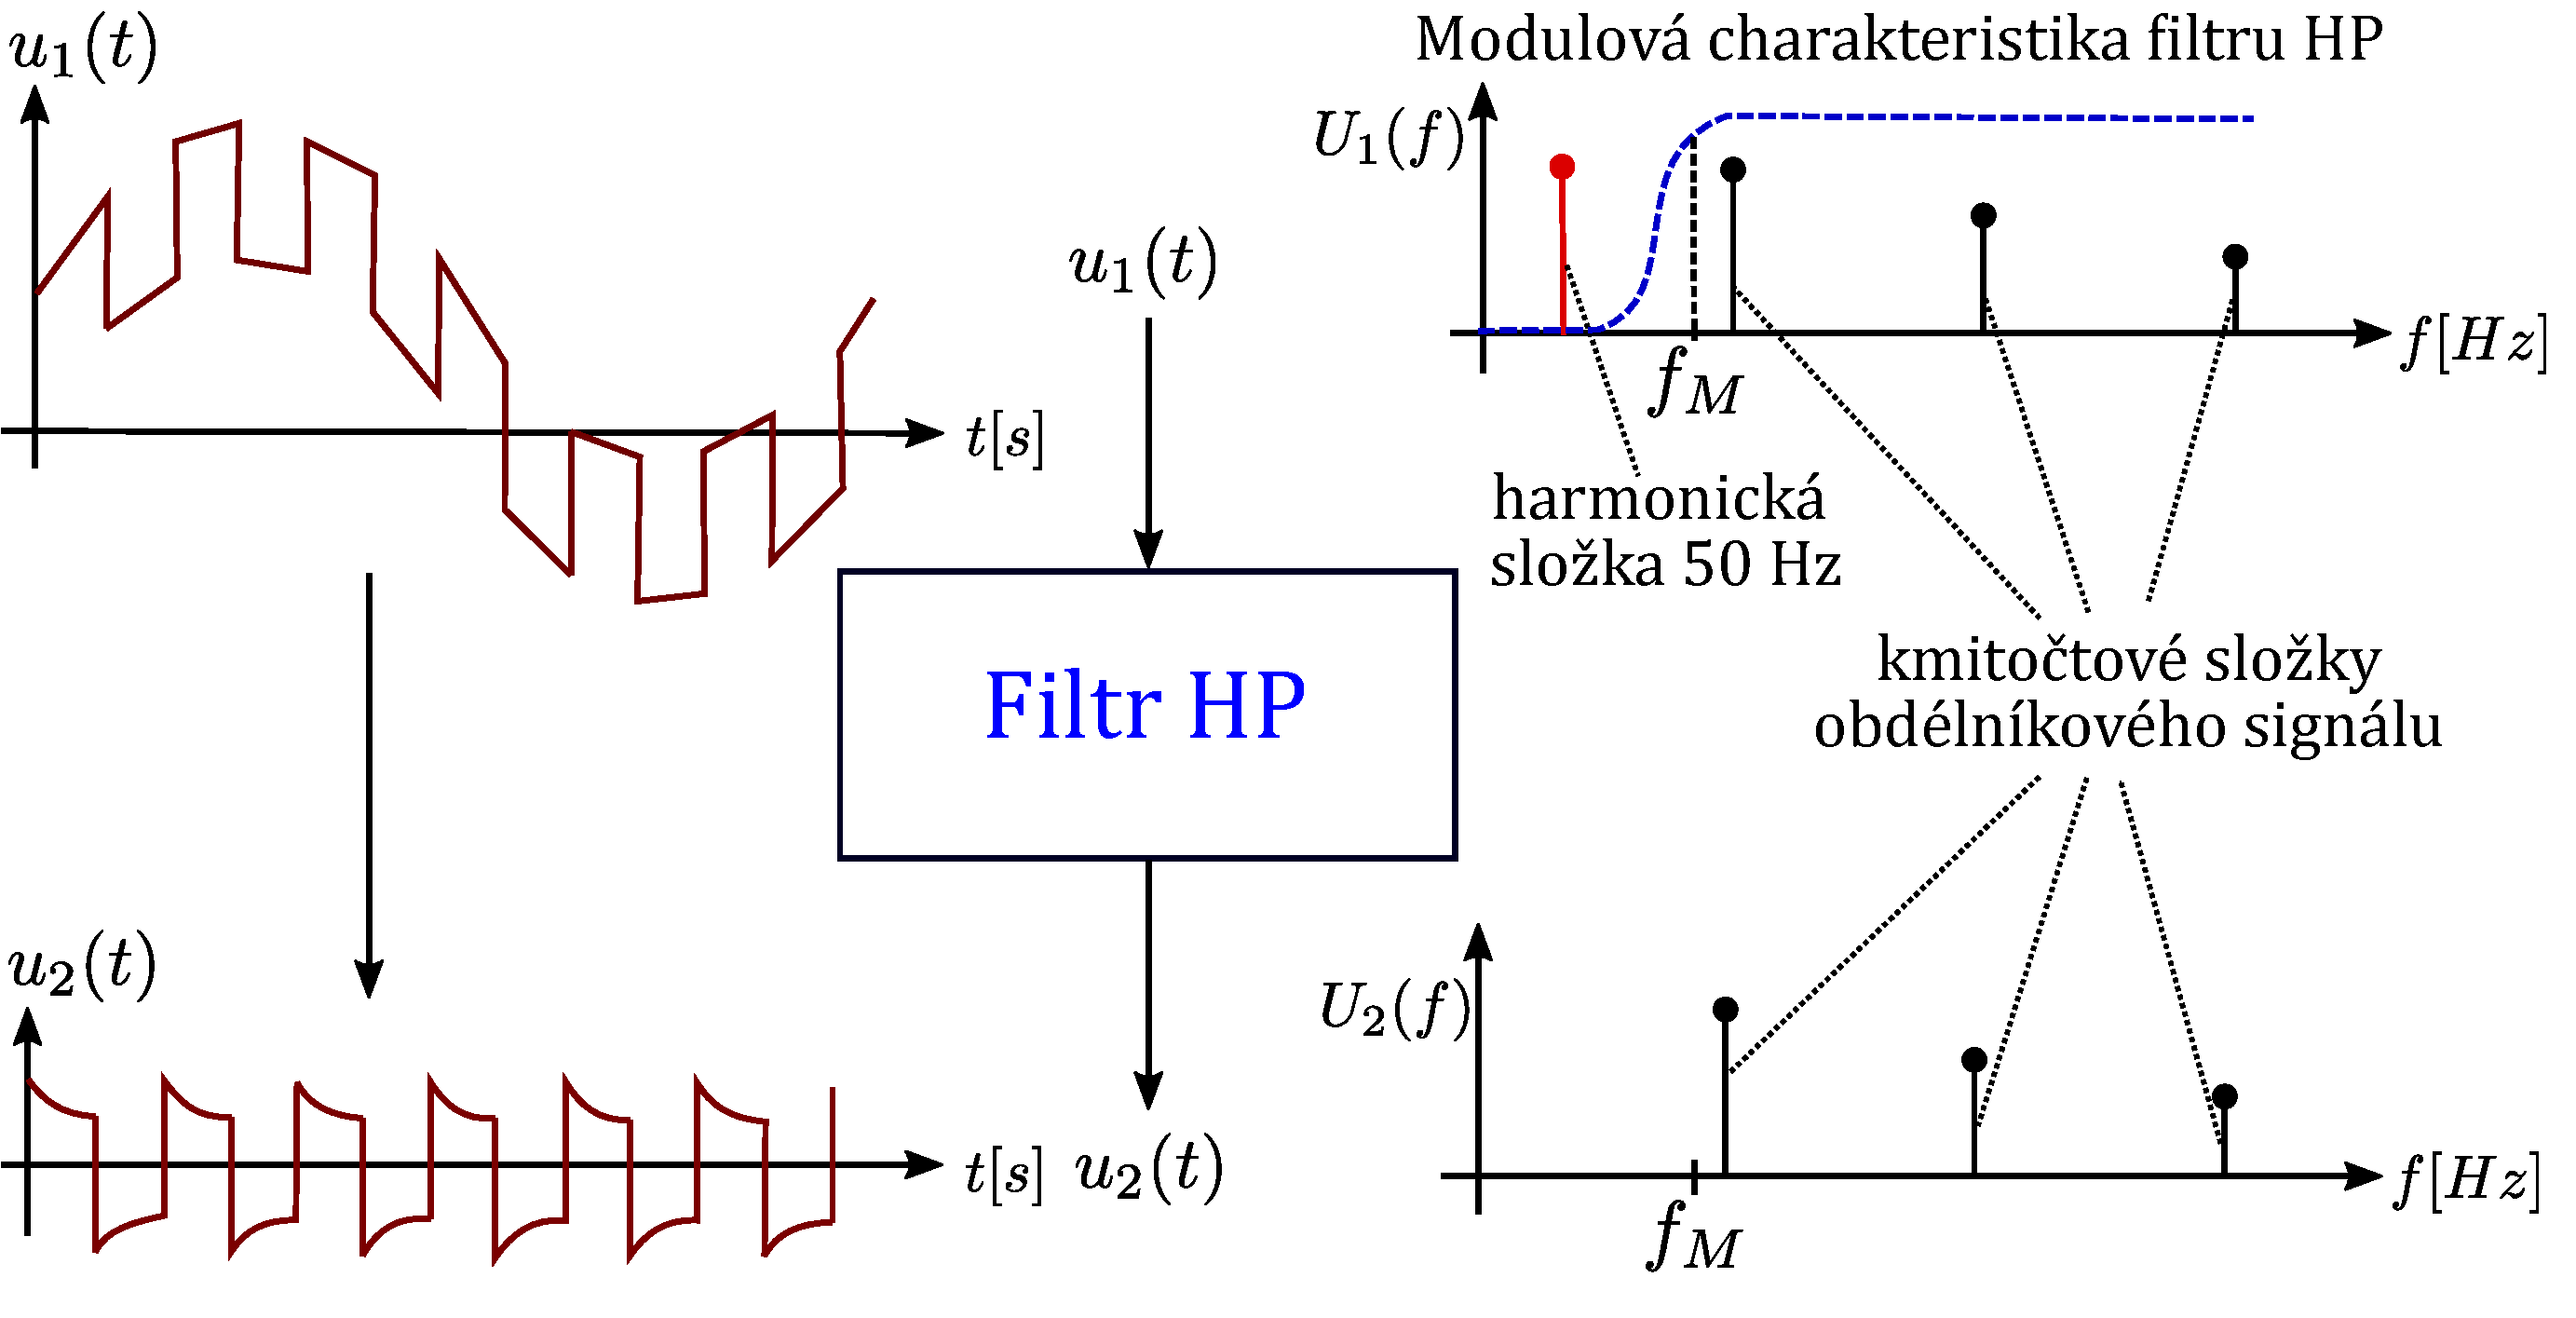
\includegraphics[width=0.8\linewidth]{aes_fig007.pdf}
      \caption{Příklad selekce kmitočtových složek signálu filtrem typu horní propust pro potlačení
                nízkofrekvenční rušivé složky (např. kmitočet sítě \SI{50}{\Hz)}
                (\cite[s.~19]{HajekSedlacek2002})}
      \label{aes:fig007}    
    \end{figure*} 
        
    \subsection{Oblasti a příklady použití}
      Kmitočtové filtry patří mezi základní stavební bloky pro zpracování signálů. V radiotechnice
      je časté použití pásmových propustí pro výběr přijímaných signálů (vstupní obvody přijímačů,
      mezifrekvenční filtry), dolních propustí a horních propustí jako výhybek pro rozdělení
      kmitočtových pásem v anténních obvodech a předzesilovačích, pásmových zádrží pro potlačení
      rušících signálů, dolních propustí pro různé typy demodulátorů atd. Moderní komunikační
      systémy s rozloženým spektrem vyžadují také jako jeden z důležitých bloků přijímače filtr typu
      pásmová propust. Obdobné je využití filtrů v telekomunikacích, při přenosu dat apod.
  
      V elektroakustice se velmi často využívají korekční filtry (nastavitelné korektory hloubek,
      výšek, pásmové korektory, korektory kmitočtových charakteristik dynamických přenosek,
      magnetofonových hlav), různé typy filtrů v systémech omezení šumu (Dolby apod ). Dolní, horní
      a pásmové propusti tvoří kmitočtové výhybky pro reproduktorové soustavy (pasivní i aktivní),
      jak ukazuje obr. \ref{aes:fig025}. V oblasti elektronické hudby se využívají i různé filtry
      pro zabarvení zvuku a realizaci zvláštních zvukových efektů.
    
      \begin{figure}[ht!]
        \centering
        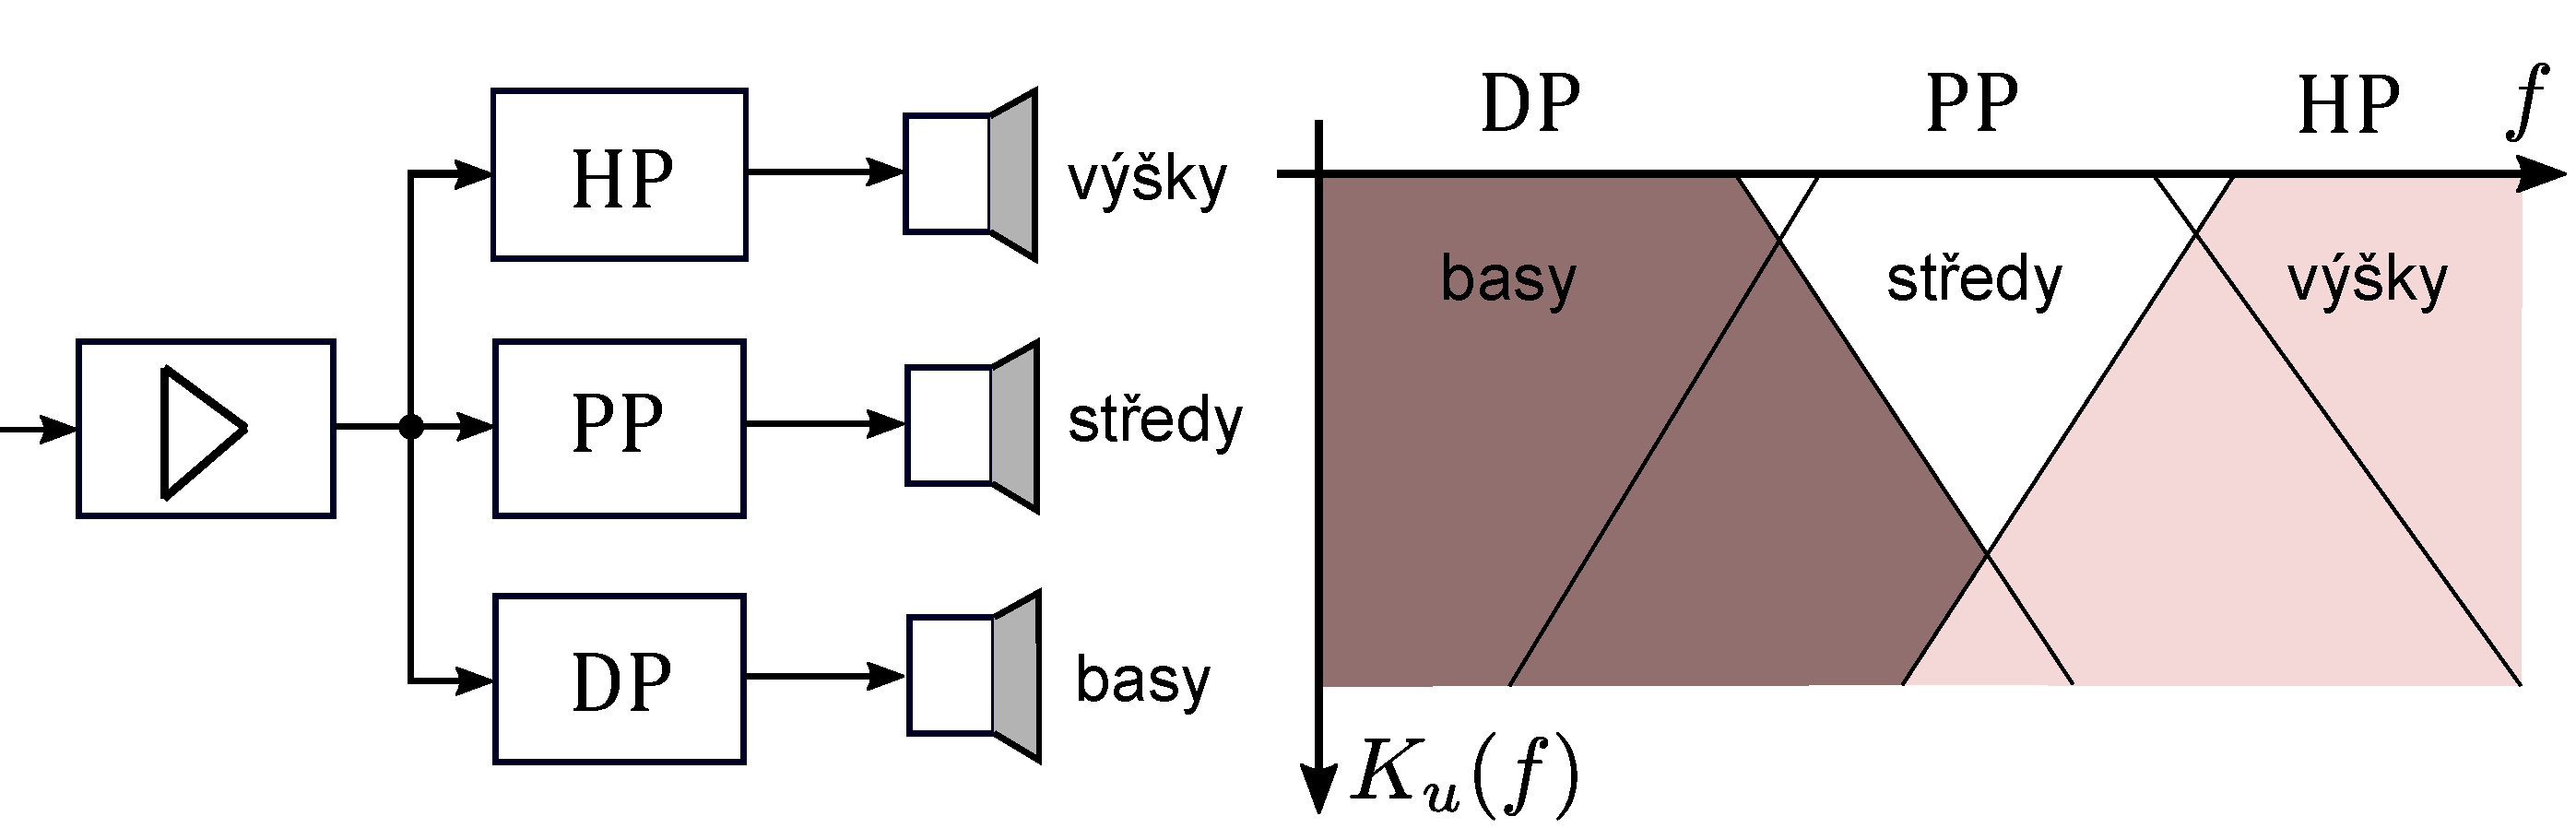
\includegraphics[width=1\linewidth]{aes_fig025.pdf}
        \caption{Příklad použití filtrů v kmitočtových výhybkách reproduktorových soustav
                 (\cite[s.~20]{HajekSedlacek2002})}
        \label{aes:fig025}    
      \end{figure} 
    
      Kmitočtové filtry se využívají také v oblasti \emph{měřicí techniky}. Velmi často jsou to
      filtry pro výběr měřeného kmitočtového pásma, obzvláště pak v různých typech selektivních
      měření (selektivní voltmetry, měřiče harmonického a dalších typů zkreslení, různá
      vysokofrekvenční měření). Pro akustická měření se využívá několika typů váhových filtrů pro
      měření úrovně akustického signálu (modeluje se vnímání lidského ucha). Často se využívá
      korektorů kmitočtových vlastností snímacích čidel. I přes rozvoj číslicových kmitočtových
      filtrů je výhodné u slabých a hodně zarušených signálů provést před A-D převodem analogovou
      předfiltraci pro podstatné zvýšení dynamického rozsahu systému.

      Zvláštní skupinu aplikací tvoří filtry typu dolní propust v systémech pro převod analogového
      signálu na číslicový. Pro splnění vzorkovacího teorému je zde v mnoha případech potřebné
      použit \emph{antialiasingový filtr} pro zamezení překládání rušivého spektra do užitečného
      signálu a na výstupu takového systému obdobný rekonstrukční filtr. Kmitočtové filtry se
      používají často v \emph{regulační technice}, speciální odrušovací filtry nacházejí uplatnění
      v \emph{silnoproudé elektrotechnice}. Takto bychom mohli vyjmenovat mnoho dalších aplikací.
      realizovat mnoha odlišnými způsoby, které do určité míry určují i některé podstatné provozní
      vlastnosti filtru. Nejvhodnější způsob realizace je potřebné si pro daný účel optimálně
      vybrat. 
    
    \subsection{Realizace kmitočtových filtrů}
      Kmitočtové filtry můžeme v praxi realizovat mnoha odlišnými způsoby, které do určité míry
      určují i některé podstatné provozní vlastnosti filtru. Nejvhodnější způsob realizace je
      potřebné si pro daný účel optimálně vybrat. Tyto způsoby realizací lze rozdělit orientačně
      do tří hlavních skupin:
      \begin{description}[noitemsep]
        \item[\textbf{diskrétní prvky}] (odpory, kondenzátory, cívky, operační zesilovače apod), kde
              si každý uživatel může s menšími či většími problémy sestavit filtr přesné podle svých
              požadavků.
        \item[\textbf{integrované bloky}] jsou obvykle menší, levnější a lépe propracované, protože 
              je výrobce vyrábí ve velkých sériích vhodnou technologii. Na druhé straně si však 
              uživatel obvykle nemůže upravit tento filtr podle svých speciálních požadavků a musí 
              přesně dodržet podmínky zapojení podle výrobce.
        \item[\textbf{číslicové filtry}] spočívají v číslicovém zpracování signálu, kdy číslicovou
              interpretaci signálu matematicky upravujeme tak, aby výsledný signál měl po zpětném
              převodu shodné (či dokonce lepší) vlastnosti jako po průchodu normálním kmitočtovým
              filtrem. Matematicky tak modelujeme požadované vlastnosti filtrů a tímto způsobem lze
              dokonce realizovat i některé funkce a vlastnosti, které běžnými analogovými filtry
              nelze dosáhnout. Při realizaci jsme však omezeni na prostředí číslicového zpracování
              signálu (převodníky, počítač či signálový procesor, vhodný program). Značným omezením
              může být i maximální rychlost výpočtu počítače a vzorkování a tím i použitelné
              kmitočtové pásmo filtru.         
      \end{description}

      Jak je z tohoto dělení zřejmé, pro optimální výběr realizace filtru neexistuje univerzální
      návod, vždy záleží na podmínkách úlohy. Jde-li o úlohu, kdy řešíme číslicové zpracování
      signálu a máme dostatečnou výpočetní kapacitu daného prostředku, zvolíme číslicový filtr. V
      jiných případech (vysoký kmitočet signálů, slabý a zarušený signál, jde-li o výkonovou
      aplikaci apod.), použijeme analogový filtr. Při tomto řešení dáváme přednost standardnímu
      integrovanému filtru profesionální výroby (např. mezifrekvenční filtry přijímačů). Pokud
      však našim požadavkům plně nevyhovuje, musíme navrhnout a vyrobit filtr požadovaných
      vlastností z dostupných diskrétních součástek. Složitost a rozmanitost vlastností
      jednotlivých realizací filtrů ukazuje i jejich následující podrobnější přehled, který
      rozděluje jednotlivé typy filtrů podle použitých stavebních prvků:

      \begin{description}[noitemsep, font=\small]
        \item[\textbf{Filtry RC}] vynikají svou jednoduchostí, dostupností a nízkou cenou výchozích
              součástek, rezistorů a kondenzátorů. Plné však u nich platí:za málo penéz - málo
              muziky. Praktické využití mají jen jednoduché filtry prvního řádu a druhého řádu s
              nízkým činitelem jakosti (\(Q < \num{0.5}\)). Filtry RC vyšších řádů se v praxi
              používají výjimečně.
        \item[\textbf{Filtry RLC}] umožňují realizovat teoreticky libovolný typ filtru. Jejich
              omezeni vyplývá především z použití cívek. Ty jsou obzvláště pro nízké kmitočty
              (velké hodnoty L) rozměrné, drahé a ztrátové (malý činitel jakosti \(Q\)). Obecné je
              také použití filtrů RLC omezeno vlastními ztrátami cívek a kondenzátorů a také
              tolerancí a stabilitou jejich hodnot pro propusti a zádrže s velmi malou relativní
              šířkou pásma. Obvykle jsou používány v kmitočtovém rozsahu od \SI{100}{\kilo\hertz}
              do \SI{300}{\mega\hertz}, pro nižší kmitočty jen výjimečné. Pro kmitočty nad
              hranicí asi \SI{300}{\mega\hertz} se výrazné projevují parazitní vlastnosti prvků a
              je lépe využít realizaci s rozprostřenými parametry - viz následující bod.
        \item[\textbf{Mikrovlnné filtry}] jsou realizací RLC filtrů v oblasti mikrovln (\(f
              \SI{>>300}{\mega\hertz}\)), kde již nelze použít prvky se soustředěnými parametry
              (R, L, C), ale používá se odpovídající realizace s rozloženými parametry jako jsou
              vlnovody, mikropásková vedení, koaxiální vedeni apod.
        \item[\textbf{Filtry ARC}] (\emph{aktivní filtry RC}) v principu nahrazují filtry RLC
              Místo cívek používají rezistory. kondenzátory a aktivní prvky, nejčastéji operační
              zesilovače. Mají obdobné vlastnosti jako filtry RLC. ale vzhledem k vlastnostem
              aktivních prvků se jejich použití omezuje nejčastéji na kmitočtové pásmo přibližné
              \SI{0.1}{\hertz} až \SI{100}{\kilo\hertz}. Současný pokrok v technologii aktivních
              prvků však umožňuje využití těchto filtrů na stále vyšších kmitočtech (dnes již
              řádové jednotky až desítky \si{\mega\hertz}), i když toto použití je zatím málo
              rozšířené. Kmitočtově jsou tedy vhodným doplňkem k filtrům RLC. Oproti nim mají
              výhodu i v snazší nastavitelnosti a laditelnosti změnou hodnot odporů. Jejich
              nevýhodou je na druhé straně potřeba napájení aktivních prvků. Objevují se i jejich
              specifické modifikace využívající parazitních vlastností aktivních prvků (R nebo C)
              jako stavebních prvků - filtry AC. AR apod.
        \item[\textbf{Filtry ASC}] (\emph{filtry se spínanými kapacitory}) jsou speciální
              modifikaci filtru ARC. které místo odporů používají přepínané kondenzátory. Jejich
              hlavní výhodou je možnost poměrně snadné monolitické integrace v porovnání s filtry
              ARC. Některé typy můžeme zakoupit jako integrované obvody. Jejich mezní kmitočet je
              určen spínacím kmitočtem a jsou tedy snadno přeladitelné. Lze je řadit již do
              skupiny integrovaných filtrů, nicméně jsou zde možnosti určitého přizpůsobení
              požadavkům, a to jednak přeladěním, jednak také dostupnosti integrovaných
              nastavitelných bloků 2. řádu. Na druhé straně je však tento typ realizace kmitočtově
              ještě více omezen než filtry ARC a má navíc problémy s vyšším driftem, s určitým
              průnikem spínacího signálu do užitečného signálu a „schodovitostí“ výsledného
              signálu, způsobenou spínáním. Spínací kmitočet bývá \(\num{50}\times\) až
              \(\num{100}\times\) vyšší než mezní kmitočet filtru, což do určité míry minimalizuje
              spínáním vzniklý projev diskretizace signálu v časové oblasti a možný aliasingový
              efekt (překládání spektra rušivého signálu do spektra užitečného signálu).
        \item[\textbf{Elektromechanické filtry}] jsou historicky nejstarší „integrované“ filtry.
              Vycházejí z principu převodu elektrického signálu na mechanický, využitím nékteré
              formy mechanické rezonance a zpětného převodu výsledného mechanického signálu na
              elektrický. Chovají se tedy vesměs jako pásmové propusti. Podle typu mechanického
              rezonátoru je lze dělit na různé skupiny. Dříve byly používány např. magnetostrikční
              filtry a dnes jsou používané nejčastěji \emph{piezokeramické filtry} (např.
              mezifrekvenčni filtry \SI{455}{\kilo\hertz} a \SI{10.7}{\mega\hertz}).
              Zvláštním typem je \emph{krystalový filtr}, který odpovídá v podstatě složenému
              rezonančnímu obvodu s vysokým činitelem jakosti (řádové \num{10000}) a vysokou
              stabilitou rezonančního kmitočtu. Nejčastěji se využívá ve stabilních oscilátorech.
              Vzhledem k vysokému a nenastavitelnému činiteli jakosti a nenastavitelnému
              rezonančnímu kmitočtu se krystaly jako filtry používají velmi omezené. Zapojením
              většího počtu krystalů s velmi přesným výběrem lze realizovat úzký pásmový filtr pro
              speciální aplikace jako např. úzkopásmové mezifrekvenčni filtry s vysokým
              rezonančním kmitočtem.
        \item[\textbf{Filtry s PAV}] (s \emph{povrchovou akustickou vlnou}, anglická zkratka SAW)
              jsou poměrné novým typem integrovaných filtrů, založených na principu vyzařování,
              šíření a fázového, kmitočtově závislého skládání povrchových akustických vln.
              Realizují se tak, že se nanese na nosnou keramickou destičku soustava vysílacích a
              přijímacích piezoelektrických zářičů, jejichž tvar a funkci lze přirovnat k dvěma
              Yagiho anténám. Obdobně jako u antén je rozměry a polohou zářičů tvarována přenosová
              kmitočtová charakteristika filtru. V porovnání s elektromechanickými filtry mohou
              realizovat podstatně širokopásmovéjší obvody. Proto se s výhodou používají, např.
              jako obrazové mezifrekvenčni filtry v televizorech a v mnoha dalších aplikacích pro
              vysoké kmitočty. Na druhou stranu je jejich použití částečné omezeno vyšším
              průchozím útlumem.
        \item[\textbf{Filtry CCD}] (\emph{charge coupled devices - nábojové vázané obvody}) jsou
              dalším speciálním typem aplikace s časové diskrétním charakterem (např. jako filtry
              ASC). Využívá se u nich technologie známá např. z CCD televizních kamer a princip
              spočívá v postupném posuvu a fázově závislém sčítání jednotlivých „nábojových
              vzorků“.
        \item[\textbf{Číslicové filtry}] jsou oproti předchozím filtrům odlišnou („softwarovou“)
              realizaci funkce filtrů, jejich princip byl popsán v předchozím odstavci.
      \end{description}
      Uvedený přehled potvrzuje značnou různorodost konečných realizací filtrů. Z přehledu
      vlastností jednotlivých typů kmitočtových filtrů je zřejmá i obtížnost úlohy konstruktéra
      při výběru optimálního způsobu realizace. Pro rychlejší orientaci o použitelnosti
      uvedených filtrů z hlediska kmitočtového pásma je možné využít tab.
      \ref{aes:fig024}. Meze použití jednotlivých způsobů realizací je nutno chápat
      jen jako orientační, protože závisí nejen na současném stavu technologie, ale i na mnoha
      různých parametrech a požadavcích kladených na filtry.

      \begin{figure}[ht!]
        \centering
        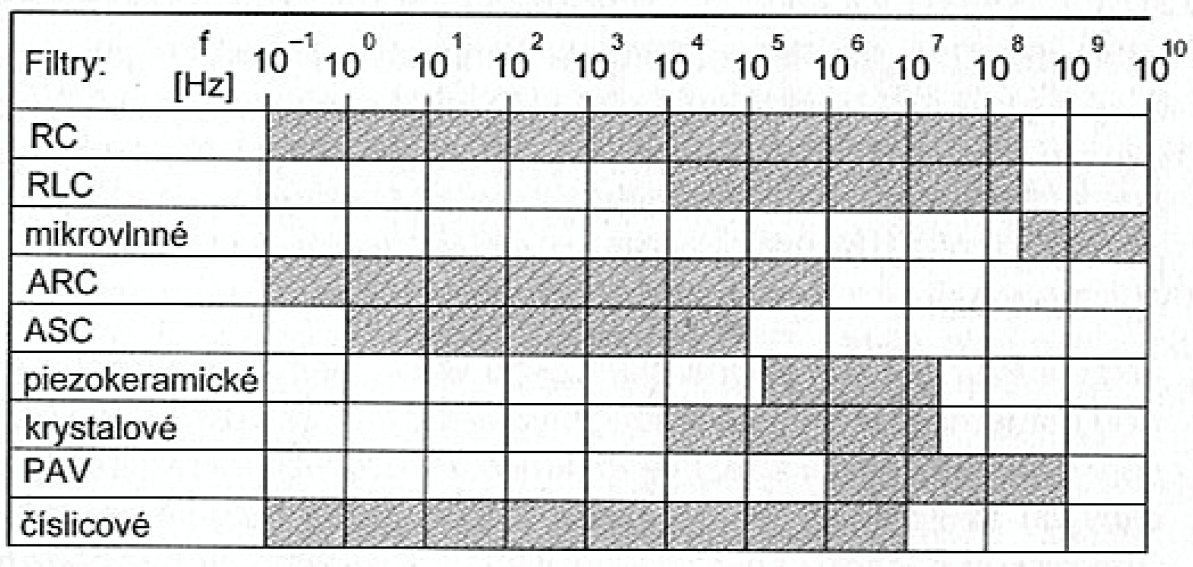
\includegraphics[width=1\linewidth]{aes_fig024.png}
        \caption{Orientační znázornění kmitočtových pásem použitelnosti jednotlivých typů realizaci
                 filtrů}
        \label{aes:fig024}    
      \end{figure} 

  \section{Popis přenosových vlastností filtrů, jejich charakteristiky}
    \subsection{Přenos filtru a průchod harmonického signálu filtrem}
      Základní zapojeni filtru připojeného ke zdroji harmonického signálu je uvedeno na obr.
      \ref{aes:fig026}. Procházi-li přes kmitočtový filtr harmonický signál s amplitudou \(U_1\),
      kmitočtem \(f_1\) a fázi \(\varphi_1\), získáme na výstupu filtru opět harmonický signál se
      stejným kmitočtem, ale jinou velikostí amplitudy a fáze (\(U_2\), \(\varphi_2\)).
  
      \begin{figure}[ht!]
        \centering
        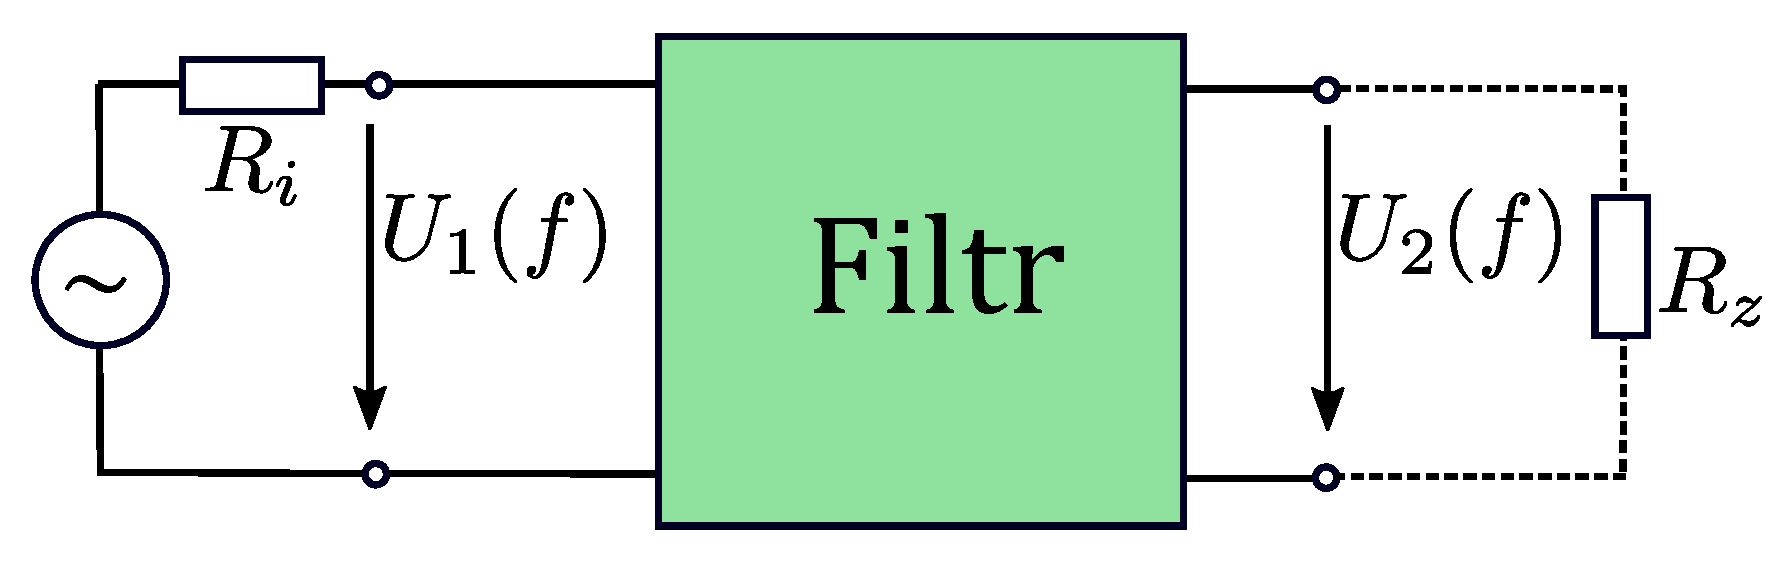
\includegraphics[width=0.9\linewidth]{aes_fig026.pdf}
        \caption{Filtr jako dvojbran (\cite[s.~25]{HajekSedlacek2002})}
        \label{aes:fig026}    
      \end{figure}
      
      \textbf{Přenos napětí} \(\mathbb{K_U}\) harmonického signálu filtrem lze pro daný kmitočet
      \(f\) vyjádřit komplexním výrazem
      \begin{equation*}
        \mathbb{K_U} = K_U\cdot e^{j\varphi} = \frac{U_2e^{j\varphi_2}}{U_1e^{j\varphi_1}},
      \end{equation*}
      který můžeme rozdělit na \emph{reálnou} a \emph{imaginární} část. Častěji ale používáme
      vyjádření přenosu pomocí \emph{modulu} a \emph{argumentu}
      \begin{equation*}
        K_U = \frac{U_2}{U_1}, \qquad \varphi = \varphi_2 - \varphi_1, 
      \end{equation*}
      kde modul \(K_U\) je poměr amplitud výstupního a vstupního signálu a argument \(\varphi\) je
      výsledný fázový posuv (časový rozdíl vztažený na periodu) mezi výstupním a vstupním signálem
      jako rozdíl fázi výstupního signálu \(\varphi_2\) a vstupního signálu \(\varphi_1\). Modul
      přenosu \(K_U\) je bezrozměrné číslo a často se udává v logaritmické míře, kdy platí \(K_U
      [\si{\decibel}] = 20 \log{K_U}\). Toto běžné používané vyjádření umožňuje grafické znázornění
      velkého rozsahu hodnot.

      Modul a argument (fázi) přenosu lze takto vypočítat jen pro konkrétní kmitočet harmonického
      signálu \(omega\). Pro praktické použití je výhodné přenosové vlastnosti vyjádřit jako funkce
      kmitočtu, kdy pro každý kmitočet lze vypočítat odpovídající přenos. Závislost přenosu na
      kmitočtu je komplexní funkcí kmitočtu \(\mathbb{K_U}(j\omega)\) či \(\mathbb{K_U}(jf)\), kde
      \(\omega = 2\pi f\) nebo \(\mathbb{K_U}(p)\), kde běžně uvažujeme \(p = j\omega\). Komplexní
      kmitočet \(p\) má obecně tvar \(p = \sigma + j\omega\) a hlubší význam (viz kap.
      \todo[inline]{1.2.5, obr, 1.16}).
      
      \begin{tcnote}  
        Dále pro zjednodušeni budeme v textu pro přenos napětí misto \(\mathbb{K_U}\) používat pouze
        symbol \(\mathbb{K}\) bez indexu \(U\), protože přenos proudu či přenos výkonu se využívá
        jen vyjimečně, např. v tzv. proudovém módu. Taktéž pro zjednodušení nebudeme rozlišovat
        komplexni přenos označením symbolem nad písmenem, ale jen uvedením proměnné jako komplexni
        \((j\omega, p)\). 
      \end{tcnote}

      Přenosová funkce má nejčastěji tvar \textbf{racionální lomené funkce} \(\mathbb{K}(j\omega)\) 
      \begin{subequations}
        \begin{align}          
            &\frac{a_m(j\omega)^m + a_{m-1}(j\omega)^{m-1} + \cdots + a_1j\omega +a_0}
                  {b_n(j\omega)^n + b_{n-1}(j\omega)^{n-1} + \cdots + b_1j\omega +b_0}  
                  \label{aes:eq027a}                                                        \\
          \shortintertext{resp. \(\mathbb{K}(p)\)} 
            &\frac{a_m(p)^m + a_{m-1}(p)^{m-1} + \cdots + a_1p +a_0}
                  {b_n(p)^n + b_{n-1}(p)^{n-1} + \cdots + b_1p +b_0} 
                  \label{aes:eq027b}
        \end{align}
      \end{subequations}      
      kde řád polynomu čitatele \(m\) je menší nebo roven řádu jmenovatele \(n\) (\(m \leq n\)).
      Tuto komplexní funkci opět můžeme rozdělit na modulovou a argumentovou část a obě veličiny
      vynést v závislosti na kmitočtu jako \emph{modulovou charakteristiku} \(K(\omega)\) a
      \emph{argumentovou kmitočtovou charakteristiku} \(\varphi(\omega)\), často také nazývanou
      amplitudovou a fázovou kmitočtovou charakteristikou (vyjádřeno z hlediska signálu) - viz obr.
      \ref{aes:fig027}. Je nutno podotknout, že v praxi je nejvíce zavedená formálně, ne zcela
      správně kombinace označení - modulová a fázová charakteristika. Vzhledem k tomu, že tato
      záměna prakticky ekvivalentních pojmů nepřináší podstatné problémy, budeme toto označení též
      používat.
      
      Příklady modulových kmitočtových charakteristik (v lineárních a logaritmických osách) pro
      ideální a reálný filtr typu dolní propust a fázové charakteristiky jsou uvedeny na obr.
      \ref{aes:fig027}. 
      
      \textbf{Velikost amplitud} jednotlivých kmitočtových složek výsledného signálu ziskáme
      vynásobením amplitud vstupních složek příslušnou velikostí modulu přenosu (např. odečteného
      z modulové kmitočtové charakteristiky filtru) pro dany kmitočet \(f\), podle vztahu
      \begin{equation*}
        U_2(f_i) = U_1(f_i)K_U(f_i).
      \end{equation*} 

      \begin{figure}[ht!]
        \centering  
        \subcaptionbox{\label{aes:fig027c}}{\luafigure[0.8]{aes_fig027c.jpg}}  \\
        \subcaptionbox{\label{aes:fig027a}}{\luafigure[0.8]{aes_fig027a.jpg}}  \\
        \subcaptionbox{\label{aes:fig027b}}{\luafigure[0.8]{aes_fig027b.jpg}}
        \caption{Příklady kmitočtových charakteristik ideálniho a reálného filtru typu dolni
                 propust: a) modulové kmitočtové charakteristiky v lineárnim měřítku, b) modulové
                 kmitočtové charakterestiky v logaritmickém měřítku, c) fázová charakteristika
                (\cite[s.~27]{HajekSedlacek2002})}
        \label{aes:fig027}
      \end{figure}

      Velikost fází kmitočtových složek výstupního signálu získáme obdobně, přičtením příslušného
      fázového posuvu filtru \(\varphi(f_i)\)) (odečteme z fázové kmitočtové charakteristiky) k
      fázím vstupních složek:
      \begin{equation*}
        \varphi(f_i) = \varphi_1(f_i) + \varphi(f_i).
      \end{equation*} 

      Obr. \ref{aes:fig028} nám tento problém ukazuje (v časové i kmitočtové oblasti) pro dva
      harmonické signály, jeden s kmitočtem \(F_a\), který leží v propustném pásmu filtru (obr.
      \ref{aes:fig028a}), a druhý s kmitočtem \(F_b\), který je v pásmu potlačení (obr.
      \ref{aes:fig028b}). Jak je zřejmé, harmonický signál s kmitočtem \(F_a\), v propustném
      pásmu prochází filtrem s minimální změnou amplitudy, pouze s určitou změnou fáze (zpoždění).
      Amplituda signálu s kmitočtem \(F_b\) v nepropustném pásmu je ale přenášena s menším
      koeficientem (viz \(K(f)\) - signál je amplitudově potlačen. Výsledná fáze signálu je (v
      souladu s fázovou charakteristikou) na tomto kmitočtu také více posunuta.
      
      \begin{figure}[ht!]
        \centering  
        \subcaptionbox{\label{aes:fig028a}}{\luafigure[0.9]{aes_fig028a.jpg}}   \\
        \subcaptionbox{\label{aes:fig028b}}{\luafigure[0.9]{aes_fig028b.jpg}}    
        \caption{Průchod harmonického signálu kmitočtovým filtrem typu dolní propust: a) signál s
                nižším kmitočtem v propustném pásmu filtru, b) signál s vyšším kmitočtem v
                nepropustném pásmu filtru (\cite[s.~28]{HajekSedlacek2002})}
        \label{aes:fig028}
      \end{figure}

      \begin{tcnote}  
        V případě, kdy je signál téměř beze změny amplitudy přenesen ze vstupu na výstup filtru
        hovoříme o \textbf{přenosu} filtru. V případě spojení filtrů se zesilovači či u filtrů ARC
        běžně dochází k zesílení signálu a mluvíme o pojmu \textbf{zisk}. Oba případy jsou
        definovány stejnou přenosovou funkcí \(K\). V případě, že je amplituda signálu na výstupu
        výrazně potlačena, se místo termínu přenos používá termín \textbf{potlačení} nebo
        \textbf{útlum}, který je převrácenou hodnotou přenosu (záporná hodnota přenosu v [dB]).
      \end{tcnote}
      
    \subsection{Průchod neharmonického signálu filtrem}
      Vliv kmitočtových a fázových charakteristik filtru na procházejici signál je dobře patrný na
      neharmonickém signálu. Obr. \ref{aes:fig029}  ukazuje v časové i kmitočtové oblasti typický
      případ - průchod obdélníkového signálu filtrem typu dolní propust (obecnější případ signálu s
      třemi různými harmonickými složkami pro různé typy ideálnich filtrů je naznačen na obr.
      \ref{aes:fig035}). Obdélníkový signál lze rozložit na základní harmonické složky. Výslednou
      amplitudu a fázi každé jednotlivé složky po průchodu filtrem můžeme vypočitat obdobně jako v
      předchozím případě obvodu s jedním harmonickým signálem - výslednou amplitudu každé harmonické
      složky určime vynásobením modulem přenosu a výslednou fázi přičtenim fázového posunu pro daný
      kmitočet (tyto hodnoty ziskáme pro daný kmitočet z modulové a fázové kmitočtové
      charakteristiky filtru). Časový průbéh vysledného signálu je potom dán součtem výsledných
      harmonických složek. Vliv modulové charakteristiky filtru na přenos signálu je zřejmý z obr
      \ref{aes:fig029}. Stejnosměrná a první harmonická složka signálu projdou filtrem typu dolní
      propust nezměněny. Vyšší harmonické složky jsou oproti nim již potlačené, což se v časové
      oblasti projevuje potlačenim ostrých hran impulzů. Poněkud komplikovanějši je situace u fázové
      charakteristiky, kdy velká nelinearita fázové charakteristiky může vést, např. až k překmitům
      a velké změně výstupniho signálu v časové oblasti. 

      \begin{figure}[ht!]
        \centering
        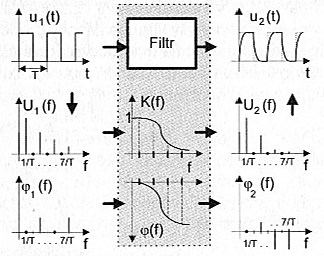
\includegraphics[width=1\linewidth]{aes_fig029.jpg}
        \caption{Průchod neharmonického signálu filtrem (\cite[s.~29]{HajekSedlacek2002})}
        \label{aes:fig029}    
      \end{figure}
    
    \subsection{Požadavky na kmitočtové charakterestiky filru} 
      Aby signál, jehož spektrum leží v propustném pásmu filtru, prošel filtrem beze změny svého
      tvaru, musí mít filtr jak konstantní modul přenosu (kmitočtově nezávislý) v propustném pásmu
      (poměr amplitud všech procházejících složek zůstane nezměněn), tak i konstantní časový posuv
      pro všechny procházející kmitočtové složky. Ze vztahu \(\varphi = \omega t\) vyplývá pro
      konstantní časový posuv požadavek lineární závislosti fázového posuvu na kmitočtu. Protože
      tato linearita se obtížně sleduje, používáme častěji kmitočtové závislosti \emph{skupinového
      (grupového) zpoždění} \(\tau_g(\omega)\) nebo \emph{fázového zpoždění} \(\tau_f(\omega)\): 
      \begin{equation*}
        \tau_g = -\der{\varphi(\omega)}{\omega}, \qquad \tau_f = \frac{\varphi(\omega)}{\omega}.
      \end{equation*}
      
      Vzhledem k tomu, že jde o zpoždění, má opačné znaménko vzhledem k přenosu fáze, přičemž
      výstupní signál je vždy opožděn oproti vstupnímu. Obě závislosti vyjadřují \emph{míru
      linearity fázové charakteristiky}, (je-li fázová charakteristika lineární, je kmitočtová
      závislost obou typů zpožděni konstantní, kmitočtově nezávislá). Jejich vzájemný vztah lze
      přirovnat k statickému a dynamickému odporu u nelineární voltampérové charakteristiky.
      Obvykle se využívá skupinového zpoždění \(\tau_g(\omega)\), fázové zpoždění
      \(\tau_f(\omega)\) se používá výjimečně. Hodnota znaménka fáze a časového posuvu závisí na
      tom, zda uvažujeme časové zpoždění či časový posuv.      
    
    \subsection{Časové charakterestiky kmitočtových filtrů}  
      V některých případech je výhodné vyjádřit vlastnosti filtru v časové oblasti, protože je v ní
      vidět přímý vliv filtru na časový průběh signálu. Typické je to např. pro sledování vlivu
      filtru na obdélnikové (číslicové) signály. Pro vyjádření vlastnosti filtrů v časové oblasti
      jsou v praxi nejčastěji používány odezvy na \textbf{jednotkový skok} \(h(t)\) (obr.
      \ref{aes:fig027b}) a na \textbf{jednotkový (Diracův) impulz} \(g(t)\). Jednotkový impulz
      je nekonečně krátký a nekonečně vysoký - je derivací jednotkového skoku. Na obr.
      \ref{aes:fig027c} je naznačen šipkou. Odezvou na tyto signály zde rozumíme časové průběhy
      signálů na výstupu obvodu po jejich přivedení na vstup obvodu. Pro uvedené časové
      charakteristiky se také používá názvů \textbf{přechodná a impulzní charakteristika}. 

      \begin{figure}[ht!]
        \centering
        \subcaptionbox{\label{aes:fig030a}}{\luafigure[0.7]{aes_fig030a.jpg}}  \\
        \subcaptionbox{\label{aes:fig030b}}{\luafigure[0.7]{aes_fig030b.jpg}}  \\
        \subcaptionbox{\label{aes:fig030c}}{\luafigure[0.7]{aes_fig030c.jpg}}  
        \caption{a) Modulová charakteristika, b) odezva na jednotkový skok (přechodná
                charakteristika), c)odezva na jednotkový impulz (impulzní charakteristika) pro filtr
                typu DP (\cite[s.~30]{HajekSedlacek2002})}
                \label{aes:fig030}
      \end{figure}
      
      Obr. \ref{aes:fig027} ukazuje příklad modulové charakteristiky filtru typu dolní propust a
      odpovídající odezvy na jednotkový skok a odezvy na jednotkový impulz, která je derivací odezvy
      na jednotkový skok. Obě časové odezvy lze vzájemné integraci či derivací převést. \emph{Odezva
      na jednotkový impulz je na rozdíl od odezvy na jednotkový skok přímým Fourierovým obrazem
      komplexní kmitočtové charakteristiky}. V praxi se vice užívá odezva na jednotkový skok,
      protože názorněji ukazuje například přenos stejnosměrné složky a můžeme z ní též dedukovat
      odezvu např. pro často používaný obdélníkový signál. 

      Popis změny tvaru obdélníkového signálu po průchodu lineárním systémem pomoci odezvy \(h(t)\)
      je obvykle definován další parametry, jako je např. \emph{maximální překmit signálu}
      \(\Delta\), \emph{doba zpoždění} \(t_z\), \emph{doba náběhu} \(t_n\) jako \emph{doba přechodu}
      z \SI{10}{\percent} na \SI{90}{\percent} úrovně signálu a \emph{doba ustálení} \(t_u\) (viz
      obr. \ref{aes:fig031}). 

      \begin{figure}[ht!]
        \centering
        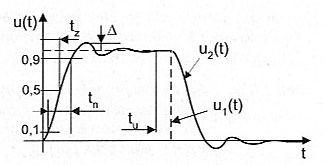
\includegraphics[width=1\linewidth]{aes_fig031.jpg}
        \caption{Průchod neharmonického signálu filtrem (\cite[s.~31]{HajekSedlacek2002})}
        \label{aes:fig031}    
      \end{figure}

      \subsubsection{Souvislosti modulových a fázových charakteristik s časovou odezvou h(t)}
        Jak již bylo naznačeno, komplexní kmitočtová přenosová funkce přímo odpovídá impulzní
        charakteristice a po integraci též přechodné charakteristice. Z přenosové funkce filtru v
        kmitočtové oblasti můžeme tedy přímo určit chování filtru v časové oblasti. 
        
        U \textbf{modulových charakteristik} platí, že velikost přenosu pro kmitočty blížící se nule
        odpovídá přenosu odezvy na jednotkový skok pro čas blížící se nekonečnu (\(K(f\rightarrow0)
        = h(t\rightarrow \infty)\) a naopak, že velikost přenosu pro kmitočty blížící se nekonečnu
        odpovídá přenosu odezvy na jednotkový skok pro čas blížící se nule \(K(f\rightarrow\infty) =
        h(t\rightarrow0)\). Proto je typická rozdílnost  průběhů odezev na jednotkový skok \(h(t)\)
        pro jednotlivé typy filtrů, jak je to znázorněno na obr. \ref{aes:fig032}. Odtud vyplývá i
        doplňkové chování jednak filtrů DP a HP a také filtrů PP a PZ. Filtr typu DP potlačuje
        ostrou náběžnou hranu jednotkového skoku a přenáší pomalé (stejnosměmé) průběhy, kdežto
        filtr typu HP naopak přenáší ostré hrany a potlačuje přenos stejnosměrné složky. Dále platí,
        že čím vyšší jsou hodnoty činitele jakosti filtru (vyšší strmost), tím více se projevuje v
        odezvě kmitavá složka. U filtru typu PP je zřejmé potlačení jak přenosu ostré náběžné hrany
        v počátku, tak i stejnosměrné složky pro čas blížící se nekonečnu. Filtr typu PZ je
        doplňkovým filtrem k filtru PP, a proto má i jeho odezva \(h(t)\) převrácený tvar, tj.
        propouští náběžnou hranu i stejnosměrnou složku a potlačuje v závislosti na hodnotě šířky
        potlačovaného pásma (činiteli jakosti) signál ve středním časovém úseku. Na obr.
        \ref{aes:fig032} je znázorněn průběh \(h(t)\) pro PZ a PP s nízkou hodnotou \(Q\) neboli
        velkou relativní šířkou pásma. V případě zužování šířky pásma může nabývat odezva charakteru
        téměř netlumeného harmonického signálu, přičemž se absolutní velikost této kmitavé složky
        snižuje.

        \begin{figure}[ht!]
          \centering  
          \subcaptionbox{\label{aes:fig032a}}{\luafigure[0.8]{aes_fig032a.jpg}}   \\
          \subcaptionbox{\label{aes:fig032b}}{\luafigure[0.8]{aes_fig032b.jpg}}   \\
          \subcaptionbox{\label{aes:fig032c}}{\luafigure[0.8]{aes_fig032c.jpg}}   \\
          \subcaptionbox{\label{aes:fig032d}}{\luafigure[0.8]{aes_fig032d.jpg}}   
          \caption{Souvislost průběhů modulových charakteristik a časové odezvy na jednotkový skok
                  pro filtry typu DP, HP, PP a PZ. Filtry typu DP a HP mají střední hodnotu \(Q\),
                  filtry typu PP a PZ nízkou hodnotu \(Q\) (relativně velkou šířku pásma)
                  (\cite[s.~32]{HajekSedlacek2002})}
                  \label{aes:fig032}
        \end{figure}

        Prakticky je také velmi důležitá souvislost případné nelinearity fázové kmitočtové
        charakteristiky a časového průběhu výstupního signálu, která je názorně vidět na přechodné
        charakteristice. 
        
        Nelinearita fázové charakteristiky filtru způsobuje i při téměř konstantní modulové
        charakteristice výrazné překmity přechodné charakteristiky, jak ukazuje příklad na obr.
        \ref{aes:fig033}. 

        \begin{figure}[ht!]
          \centering  
          \subcaptionbox{\label{aes:fig033a}}{\luafigure[1]{aes_fig033a.jpg}}      \\
          \subcaptionbox{\label{aes:fig033b}}{\luafigure[1]{aes_fig033b.jpg}}
          \caption{Souvislost průběhu fázové charakteristiky, kmitočtové závislosti skupinového
                  zpoždění a časové odezvy na jednotkový skok: a) pro téměř lineární fázovou
                  charakteristiku v propustném pásmu, b) pro nelineární fázovou charakteristiku
                  (\cite[s.~33]{HajekSedlacek2002})}
                  \label{aes:fig033}
        \end{figure}

        \begin{tcnote}
          \begin{itemize}[noitemsep]
            \item Čím důrazněji vyžadujeme zachováni tvaru procházejícího signálu, tím více musíme
                  dbát nejen na kmitočtovou nezávislost modulové charakteristiky v propustném
                  pásmu filtru, ale i na linearitu fázové charakteristiky filtru (kon- stantní
                  skupinové zpoždění). 
            \item Modulová a fázová charakteristika spolu úzce souvisí, a proto při požadavku na
                  lineární fázovou charakteristiku musíme volit odpovídající (hladký a méně strmý)
                  průběh modulové charakteristiky (viz kap. 2.3.10). 
          \end{itemize}
        \end{tcnote}

    \subsection{Základní typy filtrů}
      Jak již bylo dříve řečeno, kmitočtové filtry můžeme dělit podle různých hledisek a vlastností.
      Podle funkce filtru a odpovídajícího tvaru kmitočtových charakteristik je dělíme do tří
      základních skupin:
      \begin{enumerate}[leftmargin=0.5cm,rightmargin=1cm, label=\emph{\alph*}),noitemsep]
        \item selektivni filtry, 
        \item korekční filtry a 
        \item fázovací (zpožďovací) obvody.
      \end{enumerate}
         
      \subsubsection{Selektivní filtry}
        První skupinu tvoří filtry, které mají za úkol potlačení přenosu kmitočtových složek
        signálu v nepropustném pásmu. Podle rozložení propustného a nepropustného pásma (viz obr.
        1.11) jsou to:
        \begin{enumerate}[leftmargin=0.5cm,rightmargin=1cm, label=\emph{\alph*}),noitemsep]
          \item \textbf{dolní propust (DP)}, propouští složky signálu s kmitočty nižšími než mezní
                kmitočet \(F_M\), 
          \item \textbf{horní propust (HP)}, propouští složky signálu o kmitočtech vyšších než je
                mezní kmitočet \(F_M\), 
          \item \textbf{pásmová propust (PP)}, propouští složky signálu mezi mezním dolním a
                horním kmitočtem \(F_{M1}\) a \(F_{M2}\) 
          \item \textbf{pásmová zádrž (PZ)}, nepropouští složky signálu mezi mezním dolním a
                horním kmitočtem \(F_{M1}\) a \(F_{M2}\)    
        \end{enumerate}

        \begin{figure}[ht!]  %\ref{aes:fig034}
          \centering
          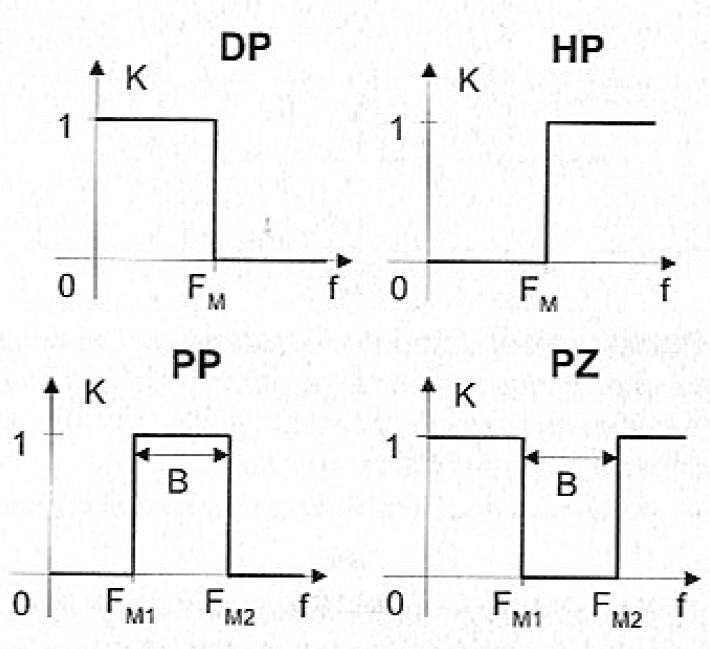
\includegraphics[width=0.8\linewidth]{aes_fig034.jpg}
          \caption{Ideální modulové charakterestiky základních typů selektivních filtrů
                    (\cite[s.~34]{HajekSedlacek2002})}
          \label{aes:fig034}    
        \end{figure}

        V ideálním případě je modul přenosu filtru v propustném pásmu konstantni (např. \(K_U = 1\)
        a v nepropustném pásmu nulový. Působení jednotlivých typů filtrů na procházející signál
        ukazuje obr. \ref{aes:fig035}, který na přikladu různých druhů signálů názorné objasňuje
        funkci a použití těchto typů filtrů. 

        \begin{figure}[ht!]  %\ref{aes:fig035}  
          \centering
          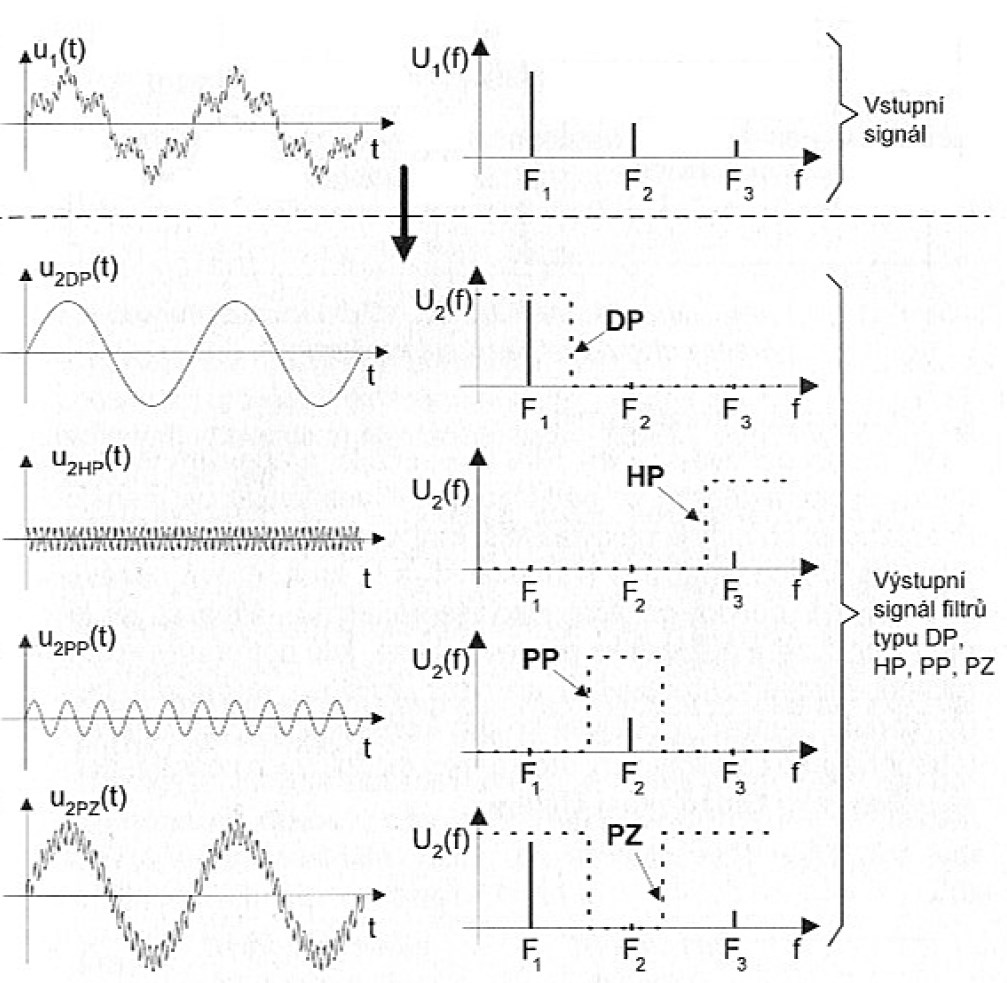
\includegraphics[width=0.9\linewidth]{aes_fig035.jpg}
          \caption{Příklad průchodu neharmonického signálu základními typy filtrů: časový průběh
                  vstupního signálu a jeho amplitudové spektrum (složen ze tří harmonických
                  signálů \(F_l\), \(F_2\) a \(F_3\)) a časové průběhy výstupních signálů a jejich
                  spektra po průchodu filtry typu DP, HP, PP a PZ
                  (\cite[s.~35]{HajekSedlacek2002})}
          \label{aes:fig035}    
        \end{figure}
        
      \subsubsection{Korekční filtry}
        Na rozdíl od předchozí skupiny selektivních filtrů je hlavním cílem těchto filtrů taková
        kmitočtová závislost přenosu \(K_2\), která koriguje přenos některých bloků přenosového
        řetězce \(K_1\) tak, aby modul přenosu celé soustavy \(K\) byl konstantní. Názorné je to v
        případě vyjádření přenosů v logaritmické míře (v dB), kdy výsledný přenos je součtem dílčích
        přenosů bloků spojených v kaskádě, jak to ukazuje obr. \ref{aes:fig036}. 

        \begin{figure}[ht!]  %\ref{aes:fig036}  
          \centering
          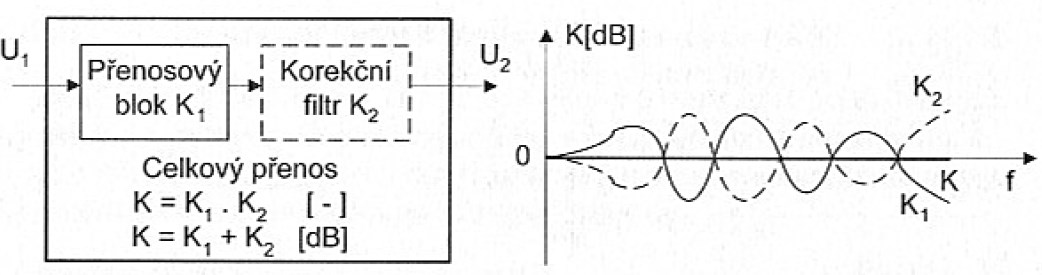
\includegraphics[width=0.9\linewidth]{aes_fig036.jpg}
          \caption{Příklad použití korekčního filtru pro korekci přenosu \(K\), tak, aby výsledný
                  modul přenosu \(K\) byl konstantní (\cite[s.~36]{HajekSedlacek2002})}
          \label{aes:fig036}    
        \end{figure}

        \subsubsection{Fázovací (zpožďovací) filtry}
          Pro předchozí dvě skupiny filtrů byly určující především vlastnosti modulových
          charakteristik, průběh fázových charakteristik byl méně důležitý. Pro fázovací obvody je
          nejdůležitější kmitočtově závislá \emph{fázová charakteristika}. Jejich modulová
          charakteristika je kmitočtově nezávislá (též se někdy tyto obvody označují jako
          všepropustné - allpass), jak je to zřejmé z obr. 1.14. Používají se především tam, kde
          potřebujeme dosáhnout různého fázového (časového) posuvu v závislosti na kmitočtu beze
          změny modulu přenosu. Používají se pro korekci fázových charakteristik (obdobně jako
          korekční filtry pro korekci modulových charakteristik) nebo se užívají jako zpožďovací
          články. 

          \begin{figure}[ht!]
            \centering  
            \subcaptionbox{\label{aes:fig037a}}{\luafigure[0.7]{aes_fig037a.jpg}}    \\
            \subcaptionbox{\label{aes:fig037b}}{\luafigure[0.7]{aes_fig037b.jpg}}    \\
            \subcaptionbox{\label{aes:fig037c}}{\luafigure[0.7]{aes_fig037c.jpg}}  
            \caption{Kmitočtové charakteristiky zpožďovacího obvodu: a) modulová, b) fázová,
                    c)skupinové zpoždění (\cite[s.~36]{HajekSedlacek2002})}
            \label{aes:fig037}
          \end{figure}

          \begin{tcnote}
            V anglosaské technické literatuře se pro označení základních typů filtrů používají jiné
            zkratky: DP - LP (\emph{low pass}), HP - HP (\emph{high-pass}), PP - BP
            (\emph{band-pass}): PZ - BR (\emph{band-reject}) a pro fázovací (všepropustný) článek FČ
            - AP (\emph{all-pass}). Dále se pro případ ostré zádrže s malou šířkou pásma používá
            pojem \emph{notch} (zářez), takže označení filtrů typu DPN (dolní propust s nulou
            přenosu - kap. \todo[inline]{missing chapter 2.2.5}) odpovídá anglická zkratka LPN
            (\emph{Iow-pass notch}).            
          \end{tcnote}

    \subsection{Řád přenosové funkce filtru a jeho praktický význam a volba}
      V předchozím textu byl uveden přenos realizovatelného filtru jako racionální lomená funkce
      kmitočtu ve tvaru
      \begin{equation}\label{aes:eq028}
        \mathbb{K}(p) = \frac{a_mp^m + a_{m-1}p^{m-1} + \cdots + a_1p +a_0}
                             {b_np^n + b_{n-1}p^{n-1} + \cdots + b_1p +b_0}
      \end{equation}
      kde \(m\leq n\). Nejvyšší mocnina \(n\) udává řád funkce a při praktické realizaci jistým
      způsobem určuje také minimální počet akumulačních prvků — cívek a kondenzátorů. Obvykle je řád
      funkce roven součtu počtu cívek a počtu kondenzátorů (viz kap. \todo[inline]{missing chap 4}). 
      
      Pro praktický návrh filtru je důležitá volba potřebného řádu filtru. Na obr. \ref{aes:fig038}
      vidíme typické závislosti modulové charakteristiky přenosu filtru typu DP pro různé řády (\(n
      = 1 \text{až} 4\). Jak je zřejmé, se stoupajícím řádem se blíží charakteristika ideálnímu
      filtru a zvyšuje se potlačení přenosu v nepropustném pásmu. Zúžuje se tak i přechodné pásmo
      mezi propustným a nepropustným pásmem. Na druhou stranu se ale zvyšuje cena a nároky na
      realizaci filtru. Proto v praktickém návrhu vždy hledáme kompromis. Z hlediska složitosti
      realizace volíme co nejnižší řád filtru, ale minimálně takový, aby zabezpečil požadované
      potlačení přenosu \(K_{POT}\) v nepropustném pásmu (pro kmitočty vyšší než \(F_P\). V uvedeném
      příkladu bychom zřejmě volili \num{3}. řád, 

      \begin{figure}[ht!]  %\ref{aes:fig038}
        \centering
        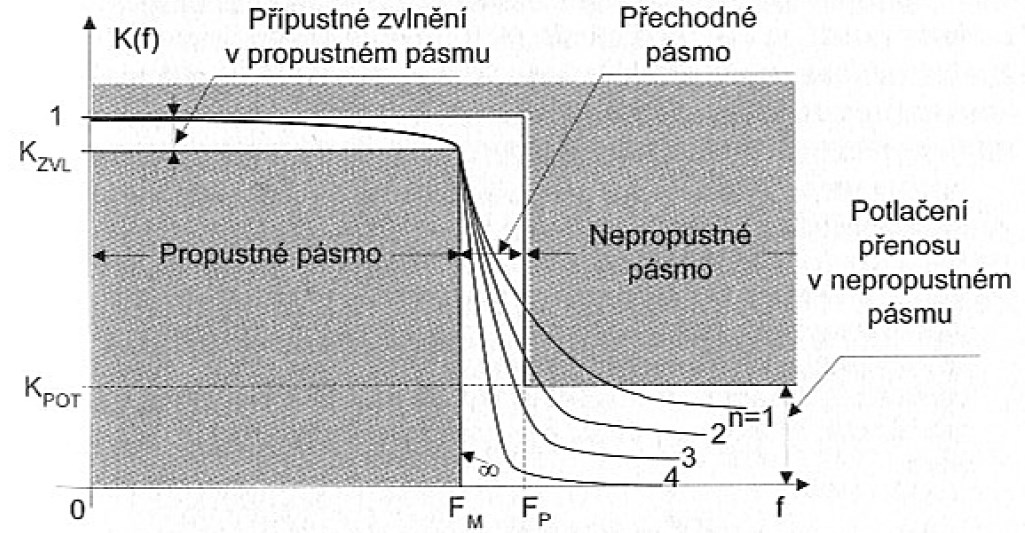
\includegraphics[width=0.8\linewidth]{aes_fig038.jpg}
        \caption{příklad závislosti modulové charakteristiky filtru typu DP na řádu filtru
                (\cite[s.~37]{HajekSedlacek2002})}
        \label{aes:fig038}    
      \end{figure}

    \subsection{Rozklad a způsoby vyjádření přenosové funkce filtru}
      Přenosové vlastnosti filtru jsou určeny v kmitočtové oblasti (ose \(j\omega\) nebo v rovině
      komplexního kmitočtu \(p\) jeho přenosovou funkcí (\ref{aes:eq027a}), resp.
      (\ref{aes:eq027b}). Určujícími parametry jsou zde koeficienty \(a_i\), a \(b_i\). Protože
      koeficienty mohou mít dosti extrémní hodnoty, je snaha normovat jejich hodnoty vůči jednomu z
      nich. Obvykle se používají dva způsoby úpravy základního tvaru prenosové funkce
      (\ref{aes:eq028}). Obě varianty rozlišíme označením koeficientů, první varianta je doplněna
      indexem 1 - \(a_{i1}, b_{i1}\), druhá indexem 2 - \(a_{i2}, b_{i2}\): 
      \begin{subequations}
        \begin{align}
          \mathbb{K}(p) 
            &= \frac{a_{m1}p^m + a_{m1-1}p^{m-1} + \cdots + a_{11}p +a_{01}}
                    {b_{n1}p^n + b_{n1-1}p^{n-1} + \cdots + b_{11}p +\textcolor{red}{1}}  
                    \label{aes:eq031a}                                                        \\
          \mathbb{K}(p) 
            &= \frac{a_{m2}(p)^m + a_{m2-1}(p)^{m-1} + \cdots + a_{12}p +a_{02}}
                    {\textcolor{red}{1}(p)^n + b_{n2-1}(p)^{n-1} + \cdots + b_{12}p +b_{02}} 
                    \label{aes:eq031b}
        \end{align}
      \end{subequations} 
      kde \(b_{01} = 1\), resp. \(b_{n2} = 1\). Pro (\ref{aes:eq031a}) plati \(a_{il} = a_i/b_0\),
      \(b_{i1} = b_i/b_0\) a pro (\ref{aes:eq031b}) plati \(a_{i2} = a_i/b_n\), \(b_{i2} =
      b_i/b_n\). Typ filtru (DP, HP, ...) určuje čitatel, rozhodující vlastnosti filtru určuje
      jmenovatel. Proto se úprava týká především jmenovatele. Používají se oba způsoby vyjádření,
      jako vhodnější se ukazuje druhý způsob, kde koeficient \(b_{02}\) vyjadřuje v podstatě mocninu
      rezonančního či mezního kmitočtu - \(\Omega_0^n\). Výhoda tohoto vyjádření je zjevná především
      pro přenosové funkce 1. a 2. řádu (viz vztah 1.12 až 1.13). V dalším budeme používat vyjádření
      podle (\ref{aes:eq031b}). Pro jednoduchost bude popis koeficientů bez doplňujících indexů, jak
      byly původně použity pro obecnou nenormovanou přenosovou funkci (\ref{aes:eq028}) - tedy
      \(a_i\), \(b_i\). 

      \begin{tcnote}
        Prakticky se používá kmitočet \(f\) v jednotkách [\si{\Hz}], ale v některých teoretických
        vypočtech je vhodnější vyjádření pomoci úhlového kmitočtu \(\omega = 2\pi f\). Kombinace
        těchto vyjádření může přinášet problémy při práci s koeficienty \(a_i\), \(b_i\)
        přenosových funkcí (\ref{aes:eq031a}) a (\ref{aes:eq031b}). Když např. vyjadřujeme
        přenosovou funkci 2. řádu (1.12) s rezonančním kmitočtem \(F_0 = \SI{1}{\kHz}\) se
        zobrazením v kmitočtových charakteristikách osou v [\si{\Hz}], musíme jako parametr
        \(b_0\) dosadit hodnotu \num{39478417.6} namisto hodnoty \num{e6}, což je dosti
        nepraktické. Přenosovou funkci s proměnou kmitočtu \(f\) [\si{Hz}] Ize vyjádřit ve tvaru 
        \begin{equation*}
          \mathbb{K}(j\omega) 
            = \frac{a'_{m}(jf)^m + a'_{m-1}(jf)^{m-1} + \cdots + a'_{1}(jf) + a'_{0}}
                  {b'_{n}(jf)^n + b'_{n-1}(jf)^{n-1} + \cdots + b'_{1}(jf) + b'_0} 
        \end{equation*}
        kde pro koeficienty platí \(a'_{m} = a_m\), \(a'_{m-1} = a_{m-1}/(2\pi)\), \(a'_{m-2} =
        a_{m-2}/(2\pi)^2\), \(\ldots\), \(a'_1=a_1/(2\pi)^{m-1}\), \(a'_0=a_0/(2\pi)^{m}\) a
        obdobně \(b'_n = b_n\), \(b'_{n-1} = b_{n-1}/(2\pi)\), \(b'_{n-2} = b_{n-2}/(2\pi)^{2}\),
        \(\ldots\), \(b'_{1} = b_{1}/(2\pi)^{n-1}\), \(b'_0 = b_0/(2\pi)^n\). Při výpočtu přenosu
        tak lze pracovat s dvěma odlišnými typy koeficientů.
      \end{tcnote}
 
      \subsubsection{Rozklad přenosové funkce filtru pomocí pólů a nul přenosu v komplexní rovině p}
        Protože z hodnot koeficientů přenosových funkcí vyšších řádů nejsou přenosové vlastnosti
        filtru dobře patrné, je snaha rozložit tyto funkce na dílčí funkce nižších řádů. K tomuto
        rozkladu vedou i potřeby některých návrhových postupů pro realizaci filtrů. Nejčastěji se
        přenosová funkce upravuje pomocí rozkladu polynomů čitatele a jmenovatele na kořenové
        činitele do tvaru
        \begin{align}\label{aes:eq032}
          \mathbb{K}(p) 
            &= \frac{a_{m}(p)^m + a_{m-1}(p)^{m-1} + \cdots + a_{1}p +a_{0}}
                    {(p)^n + b_{n-1}(p)^{n-1} + \cdots + b_{1}p +b_{0}}          \nonumber\\
            &= \frac{(p-p_{am})(p-p_{a(m-1)})\cdots(p-p_{a1})}
                    {(p-p_{bm})(p-p_{b(m-1)})\cdots(p-p_{b1})},                  
        \end{align}
        kde \(p_{ai}\) jsou obecně komplexní kořeny polynomu čitatele a \(p_bi\) jsou obecně
        komplexní kořeny polynomu jmenovatele v rovině \(p\). Dosadíme-li za hodnotu komplexního
        kmitočtu \(p\) jeden z kořenů čitatele \(p_{ai}\), bude hodnota příslušného členu a tudíž i
        celého čitatele a přenosové funkce nulová. Potom hovoříme o \textbf{nulovém bodu funkce}
        (\emph{vyjadřuje nulový přenos}). Dosadíme-li za \(p\) obdobně jeden z kořenů jmenovatele
        \(p_{bi}\) bude hodnota celého jmenovatele nulová a přenosová funkce bude mít v tomto bodě
        nekonečnou hodnotu, jedná se o tzv. \textbf{pól přenosové funkce} (\emph{vyjadřuje nekonečný
        přenos}). 
        
        Dále je potřebné si uvědomit, že některé z koeficientů čitatele \(a_0\), až \(a_m\) mohou
        být a obvykle bývají nulové (tím je určen typ filtru, např. DP, HP). tudíž počet kořenů
        čitatele \(p_{ai}\) může být nižší, či mohou mít nulovou hodnotu. Oproti tomu \emph{všechny
        koeficienty jmenovatele musí být vždy nenulové a kladné a kořeny \(p_{bi}\) musí být vždy
        nenulové a se zápornou reálnou částí}. 
        
        Jednoduchý příklad přenosové funkce druhého řádu s nulou přenosu (filtr DPN - viz kap.
        \todo[inline]{ kap 2.2.5 is missing}) je ukázán na obr. \ref{aes:fig040}. Přenosová funkce
        komplexní proměnné \(p\) (rov. \ref{aes:eq032}) je znázorněna jednak jako trojrozměrná
        funkce (obr. \ref{aes:fig040a}), dále pak obvyklejší dvojrozměrnou formou průmětu pólů a
        nulových bodů přenosu v komplexní rovině \(p\) (obr. \ref{aes:fig040b}). Důležité je, že
        póly i nulové body přenosu se vyskytují v komplexně sdružených dvojicích (pouze v případé
        přenosové funkce lichého řádu je odpovídající nulový bod a pól vždy jeden a reálný). Dále je
        zřejmé, že další běžně použivané dvourozměrné vyjádření - modulová charakteristika prenosové
        funkce v ose \(j\omega\) (obr. \ref{aes:fig040c}), je řezem přenosové funkce v komplexní
        rovině \(p\) (uvažuje se jen kladná poloosa \(j\omega\)).        
        
        Za povšimnutí stojí, že póly s nekonečným přenosem vzhledem k nutné poloze vlevo od osy se
        promítají do kmitočtové charakteristiky jen určitým navýšením přenosu (závislým na hodnotě
        \(Q\) - čim vyšší \(Q\), tim blíže osy), kdežto nulové body jsou obvykle umístěny přímo na
        ose \(j\omega\) a tudíž se promítnou jako minima (nuly) přenosu v kmitočtové
        charakteristice. Protože většinou budeme využívat zobrazení v kmitočtové ose, budeme dále
        pro jednoduchost používat označení \emph{nuly přenosu}. 

        \begin{align}\label{aes:eq035}
          \mathbb{K}(p) 
            &= \frac{\Omega_0^2}{\Omega_N}\cdot
               \frac{p^2 + \Omega_N^2}{p^2 + p\Omega_0/Q + \Omega_N^2}     \nonumber \\
            &=\num{0.585}\frac{p^2 + 4}{p^2 + \num{0.6}p + \num{2.34}}     \nonumber \\
            &=\num{0.585}\frac{(p-j2)(p+j2)}{(p+\num{0.3}-j\num{1.5})(p+\num{0.3}+j\num{1.5})}            
        \end{align}

        \begin{figure}[ht!]
          \centering  
          \subcaptionbox{\label{aes:fig040a}}{\luafigure[0.7]{aes_fig040a.jpg}}         \\
          \subcaptionbox{\label{aes:fig040b}}{\luafigure[0.7]{aes_fig040b.jpg}}         \\
          \subcaptionbox{\label{aes:fig040c}}{\luafigure[0.7]{aes_fig040c.jpg}}  
          \caption{Příklady komplexní přenosové funkce 2. řádu typu DPN a způsoby jejího grafického
                  znázornění: a) trojrozměrně, b) průměty pólů a nulových bodů přenosu v komplexní
                  rovině \(p\), c) modulová charakteristika jako řez trojrozměrné funkce v rovině
                  \(j\omega\) (pro \(\sigma = 0\)) s nulou přenosu
                  (\cite[s.~40]{HajekSedlacek2002})}
          \label{aes:fig040}
        \end{figure}

        \subsubsection{Rozklad celé přenosové funkce pomocí přenosových funkcí 1. a 2. řádu v
                       kmitočtové oblasti}
          
          Uvedený způsob znázornění přenosové funkce v rovině \(p\) je velmi zajímavý a potřebný
          především pro teoretickou práci. Pro běžnou práci s kmitočtovými filtry je praktičtější
          následující způsob rozkladu. Vychází z poznatku, že přenos komplexně sdružené dvojice pólů
          a nul lze vyjádřit přenosovou funkcí 2. řádu jak pomocí proměnné \(j\omega\)
          [\si{\radian\per\sec}], tak i po přepočtu méně používaným, ale názornějším způsobem pomocí
          proměnné \(jf\) [\si{\Hz}] (viz poznámka v úvodu této kapitoly) 
          \begin{align}\label{aes:eq033}
            \frac{(p-p_{ai})(p-p_{ai})}{(p-p_{bi})(p-p_{bi})}
              &= \frac{p^2 + a_{i1}p + a_{i0}}{p^2 + b_{i1}p + b_{i0}}          \nonumber \\ 
              &= \frac{p^2 + p\dfrac{\Omega_{Ni}}{\Omega_{Ni}} +\Omega^2_{Ni}}
                      {p^2 + p\dfrac{\Omega_{0i}}{\Omega_{i}} +\Omega^2_{0i}}        
          \end{align}
          \begin{align}\label{aes:eq040}   
            &\Leftrightarrow
             \frac{(j\omega)^2 + j\omega\dfrac{\Omega_{Ni}}{\Omega_{Ni}} +\Omega^2_{Ni}}
                  {(j\omega)^2 + j\omega\dfrac{\Omega_{0i}}{\Omega_{i}} +\Omega^2_{0i}}
            =\frac{-\omega^2   + j\omega\dfrac{\Omega_{Ni}}{\Omega_{Ni}} +\Omega^2_{Ni}}
                  {-\omega^2   + j\omega\dfrac{\Omega_{0i}}{\Omega_{i}} +\Omega^2_{0i}} \nonumber \\   
            &\Leftrightarrow
              \frac{(jf)^2 + jf\dfrac{F_{Ni}}{Q_{Ni}} + F^2_{Ni}}
                   {(jf)^2 + jf\dfrac{F_{0i}}{Q_{i}}  + F^2_{0i}}
            = \frac{-f^2   + jf\dfrac{F_{Ni}}{Q_{Ni}} + F^2_{Ni}}
                   {-f^2   + jf\dfrac{F_{0i}}{Q_{i}}  + F^2_{0i}}. 
          \end{align}
          Obdobně pro 1. řád platí
          \begin{equation}\label{aes:eq034}
            \frac{(p-p_{ai})}{(p-p_{bi})} = \frac{p + \Omega_N}{p + \Omega_0} \Leftrightarrow
            \frac{j\omega + \Omega_N}{j\omega + \Omega_0}\quad\text{resp.}\quad
            \frac{jf + F_N}{jf + F_0}.
          \end{equation}
                    
          Z uvedených vztahů vyplývá, že u \emph{jmenovatelů přenosových funkcí} prvního řádu
          vystupuje jeden parametr - mezní kmitočet \(\Omega_0\), resp. \(F_0\) a u druhého řádu dva
          parametry-rezonanční kmitočet \(\Omega_0\), resp. \(F_0\) a \emph{činitel jakosti} \(Q\).
          Tyto parametry mají zjevný fyzikální význam (\todo[inline]{viz kap. 2.1, 2.2}) a jsou
          velmi často používány. 
          
          \emph{Čitatel přenosové funkce} musí mít jeden koeficient nenulový, ostatní koeficienty
          mívají obvykle nulovou hodnotu (tomu odpovídá poloha nulových bodů přenosu v nule, či
          nekonečnu). Tím je určen typ filtru (DP, HP, PP - \todo[inline]{viz kap. 2.2}). V případě
          filtru 2. řádu typu pásmová zádrž (či jeho variant DPN nebo HPN) je nulový koeficient
          pouze jeden, a to \(Q_N = \infty\) neboli \(a_{i1} = 0\). Pak má kmitočet nuly přenosu
          \(\Omega_N\), resp. \(F_N\) konečnou hodnotu, zjevný fyzikální význam a v komplexní rovině
          se vyskytuje pouze na ose \(j\omega\) (viz obr. \ref{aes:fig040}). Podrobněji opět v kap.
          \todo[inline]{viz kap. 2.2}. Po dosazení rovnice (\ref{aes:eq033}) do přenosové funkce
          vyššího řádu (\ref{aes:eq035}) dostaneme pro sudý řád \(n\) při úhlovém kmitočtu
          \(\omega\) V [\si{\radian\per\sec}] přenosovou funkci ve tvaru součinu \(n/2\) přenosových
          funkcí 2. řádu
          

  \section{Obecný postup při návrhu kmitočtových filtrů}
    \begin{figure}[ht!]  %\ref{aes:fig039}
      \centering
      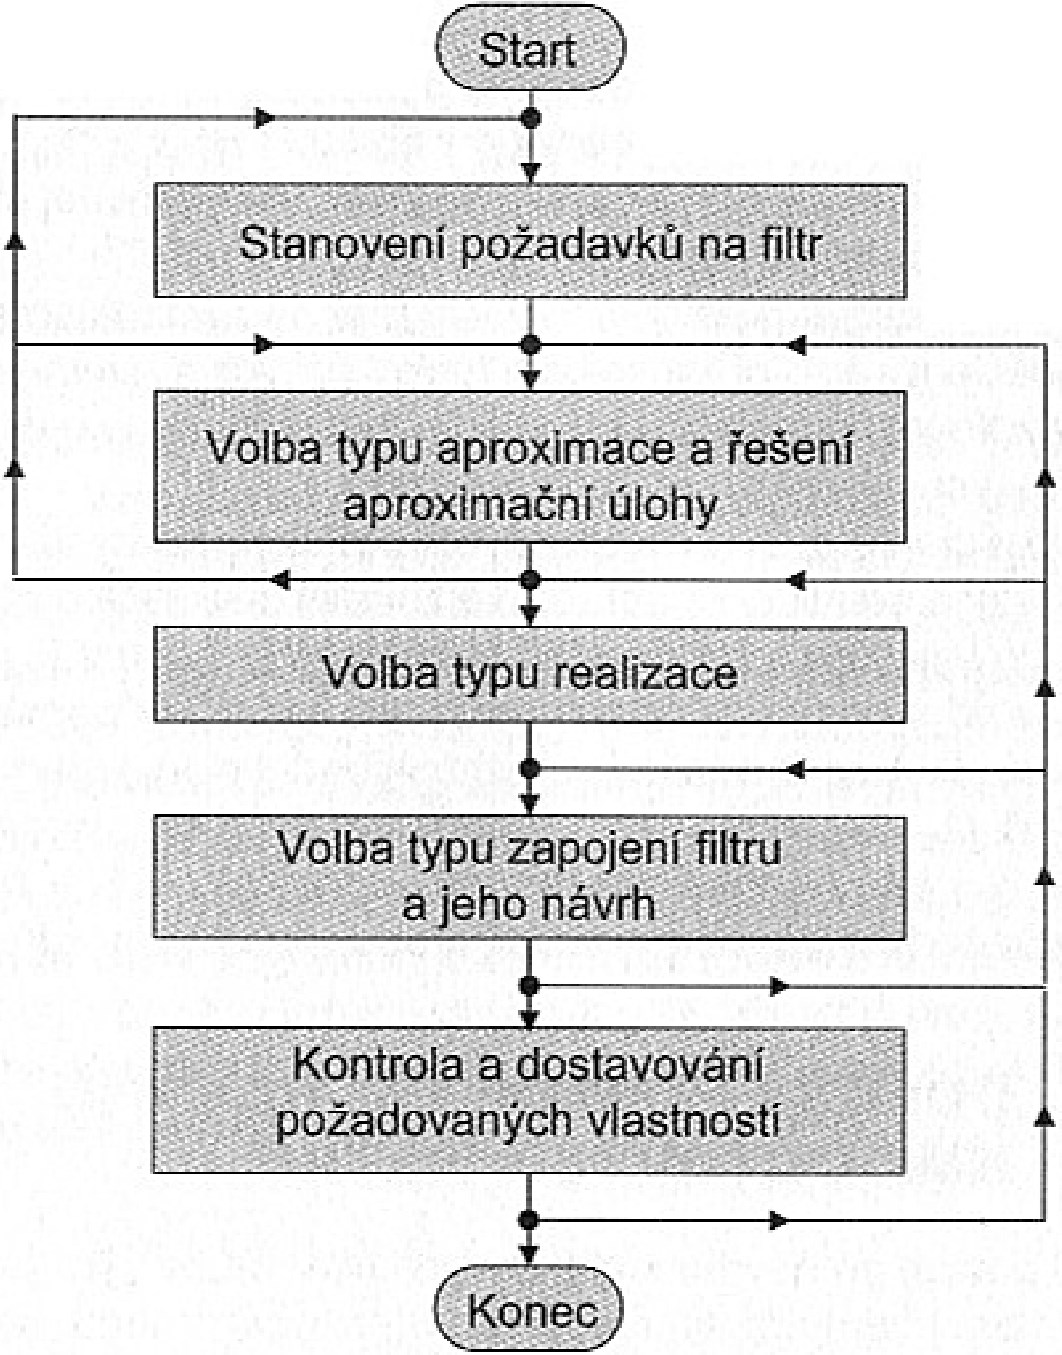
\includegraphics[width=0.8\linewidth]{aes_fig039.jpg}
      \caption{Diagram možného postupu při návrhu kmitočtových filtrů
              (\cite[s.~44]{HajekSedlacek2002})}
      \label{aes:fig039}    
    \end{figure}

%---------------------------------------------------------------------------------------------------